\chapter{设计}

% 4.1

\section{设计概述}
在这小节中,我们将要简要讨论整个同步过程。后面的章节将会详细讲述同步的各个部分的细节。

\subsection{树形拓扑}

当有人要加入这个系统,他要做的第一件事就是在系统的拓扑中找到一个位置。
一般的,在最初阶段,每一个人都要找到自己的位置。
每个人会等待一个随机的时间,然后发送“Any Server Interest”请求。
如果他没有收到回复,他将会假设自己是控制器,所以能够去回复别人的“Any Server Interest”请求。
当收到这种回复时,参与者会将他所在节点的父节点设置为收到回复的发起者,并向他索要同步控制信息。
“Any Server Insterest”是和特定层级相关的,这是为多层树结构做准备。

每一个人都要发送心跳包来确定自己的控制节点是否还存在。
一旦检测到其控制节点宕机了,或者由于什么原因下线了,
一个新的控制器会从这个控制器所管辖的客户中选出一个,接替它的位子。
当然,一个新的参与者可以很容易的从他的附近找到一个节点当做自己的控制节点。

\subsection{控制信息}
控制器通过向自己的子节点发送控制信息来主导同步过程。
控制信息并不是真正的数据,而是一种包含什么时间在什么地方有新数据的信息包。
它会告诉接收者,应该在正确的时间到正确的地点拿取数据。
此包中除了包含真正消息的NDN名字,还包含一个标签。
当控制信息顺着拓扑树向下传播时,每一层的控制器都会将自己的名字和他当前的时间加入这个标签。
最终结果是,节点收到的控制信息包中将会包含它上层所有的控制器的名字和时间信息。

\subsection{同步}

当一个节点产生消息,或者更一般的,知道一些新的东西需要向群体中传递,他将会沿着拓扑树向上和向下传递。

向上传递。
当一个节点有新消息要发布,它想他的父节点,也就是他的控制器发送一个带有实际消息名称的Interest。
当控制器收到这个Interest,他将自己的名字和时间添加到这个记录的标签中,然后把它存储在自己本地的日志中。
如果他还有上层节点,它会按照同样的方式向上传递。

向下传递。
为了得到最新的控制信息,每一个用户都会定期向他的控制器发送同步兴趣包,我们称之为“Anything New Interest”。
该包中包含他所知道的最新的标签信息。当一个同步兴趣包超时了,用户会重发此兴趣包。
当控制节点收到该兴趣包后,会和自己的当前知道的最新的标签进行比较。
\begin{enumerate}
  \item 如果标签的时间和他自己的时间是一样的,说明现在他和客户的状态是相同的,此时不需要传递控制信息。
  控制节点会把这个兴趣包保留,以便以后有新的信息时能够迅速响应。
  \item 如果这个标签比他自己的更早,说明该客户的状态已经旧了,需要更新。这时候,他会将用户标签时间点之后的所有新的记录返回给该用户。
  当收到同步兴趣包的返回结果后,客户端会将这个消息记录在自己的日志中,并更新自己的状态。
  这时候他的状态会比他保留的同步兴趣包新,所以会按照相同的方式,继续将此消息向他的子节点传递。
  从而可以达到将控制信息转发给全局的目的。
\end{enumerate}

\subsection{实际消息本体的获取}

当收到控制信息后,每个人都会知道新的消息的NDN名字。
他们直接发送数据请求兴趣包,去向消息产生者索取消息实体。
因为数据的名字在NDN中是唯一的而且稳定不变的,每个参与者的发送的索取相同信息的兴趣包是相同的,
那么这些兴趣包就会被路由聚集,并只发送一份兴趣包的拷贝去下一跳路由。
这就保证了每一个链路中相同的兴趣包只有一个,而不会有重复。当这个兴趣包达到消息产生者后,他会返回消息实体。
此数据包会沿着兴趣包相反的路径传递到所有发送兴趣包的用户,因此overhead非常小。
同时,返回的数据包可以被路由器缓存到本地的内存中,所以当之后有用户请求相同的数据,
他将会直接从临近的路由的缓存里面拿,而不是从消息的产生者那拿。




% 4.2

\section{命名规则}

\begin{table}
\renewcommand{\arraystretch}{1.3}
\caption{Interests' Names}
\label{interest_name}
\centering
\begin{tabular}{|c|c|}
\hline
Any Server Interest & /broadcast/treesync/anyserver/\emph{level}\\
\hline
Something New Interest & /\emph{serverName}/treesync/somethingnew/\emph{mylabel}/\emph{dataName}\\
\hline
Anything New Interest & /\emph{serverName}/treesync/anythingnew/\emph{label1:label2:label3}\\
\hline
Data Interest & /\emph{publisherName}/treesync/\emph{time}\\
\hline
\end{tabular}
\end{table}

命名是NDN应用程序最重要的部分之一,因为NDN的本质是以名字命名数据。
在这一章,我们简要描述我们在设计中所使用的所有兴趣包的名字。
后面的章节将会分别详细讲述这些兴趣包的用途。

我们的设计中总共有四中兴趣包的名字。
Anything New Interest 用于产生控制器树形拓扑。
Something New Interest 和 Anything New Interest 用于控制消息的传输。
Data Interest 用来获取真正的消息实体。

名称的第一部分是为了保证路由可以正确的转发它们。
’/broadcast’的兴趣包会被路由到所有相关的端口。
’/serverName’和’/publisher’的兴趣包会被路由到指定的节点。

第二部分’/treesync’是标志当前应用程序的标签。

其他的成分是和具体流程相关的,我们将在后面几章分别讨论。

%4.3

\section{树形拓扑产生}

\begin{figure}
\centering
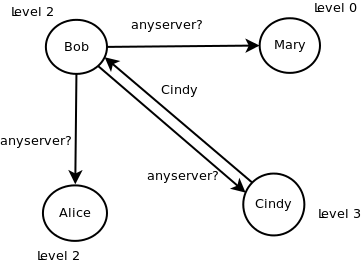
\includegraphics[width=4.5in]{png/server-generation.png}
\caption{Server Generation}
\label{server_generation}
\end{figure}

为了产生控制器,我们将使用“Anything New Interest”。
名字的前两部分是为了路由传输和应用处理兴趣包。
第三个部分是兴趣包的类型。
最后一个元素“level”是一个数字,代表了当前这个兴趣包所使用的控制器层级。

在开始阶段,每个人都是独立的没有控制器的。
它们会各自等待一个随机的时间,然后向所有聊天用户广播一个ASI来询问周围有没有控制器。
然后他们会等待一个特定时间Ts。
如果能在Ts过期前收到返回的数据包,它就会将返回此包的用户作为他的父节点,然后发送给他同步兴趣包来索取控制信息。

如果他没有在Ts过期前收到回复,他就会将自己作为一个控制节点,并且准备好回复别的节点的相同的请求。
当区域很大时,在所有一级控制节点之上,会产生更高层的控制节点。
这些节点的生成和之前的算法一样,只是在等待时间上,会和其层级相关,更大的等待时间可以生成更大的区域。
如果在到期之前没有收到回复,控制器就将自己的层级加一。

我们设置一个小的整数,作为最高层级。
只要一个参与者没有上层控制器,而且自己不是最高层控制器,他就会进行这个产生过程。
如果一个节点已经有控制节点,他会向该节点定期发送心跳兴趣包来检测该节点的有效性。
我们将在第七节讨论节点宕机的处理。

注意到控制节点的产生过程和实际拓扑是息息相关的,信息传递的方向当然也是和拓扑相关的。
这就使得经过控制器的延迟不会比直接传递的延迟有显著的增加。
从而保证了传输时延性能。



\section{同步过程}

\begin{figure}
\centering
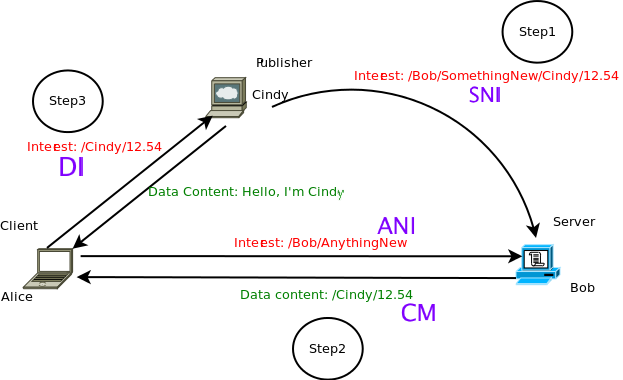
\includegraphics[width=4.5in]{png/synchronization.png}
\caption{Synchronization and Data Fetching}
\label{synchronization}
\end{figure}


本章,我们将描述在系统中到底是如何同步的。
如图所示,子节点向其父节点发送SNI来通知他有一个新的消息。
控制节点然后会回复他保存的待决定的ANI,其中包含这个新的消息。
参与者通过分布式的方式获取消息实体。图4显示了多层拓扑的同步。
每个节点都会通过发送SNI和满足ANI来向上和向下传递控制信息。

\subsection{Something New Interest}
当一个节点产生一个新的消息,或者他收到来自下层节点的SNI,他会将此消息向上传递给自己的控制节点。

当一个参与者产生一个新的数据,他将会做下面这些事:
\begin{enumerate}
  \item 添加这个数据进入自己本地的数据存储器
  \item 将自己的标签加入这条记录中,并且将这条记录放入自己的记录存储器。
  \item 向他的控制节点发送SNI,其中包含他的标签和实际数据的NDN名字。
  \item 处理来自子节点的待处理的ANY
\end{enumerate}

注意到SNI在其后面包含了真是的数据名字,所以当控制节点收到此SNI后,他可以立即将这个消息向上或者向下传递。

\subsection{Anything New Interest}
为了得到控制信息,每一个节点都会周期性的向他的控制节点发送带有他当前最新标签的ANI。
当一个控制节点收到这个兴趣包时,他会将其中包含的标签信息和他自己的最新标签做对比。
有如下三种情形:
\begin{enumerate}
  \item 此标签和他自己的标签时间相同。
这时候,他将会把这个兴趣包保留为待处理的同步兴趣包,这样能够在他有状态变化时第一时间将此变化回复给其客户端。
  \item 收到的兴趣包中包含的标签晚于自己当前的标签。
这时候,他比较这个记录的时间,找到本地记录中所有比此标签新的记录,然后将所有记录返回给该兴趣包。
  \item 在自己的记录中没有此标签对应的用户信息。
这种情况下,需要将所有的记录都发送给子节点。
\end{enumerate}

当子节点收到ANI的数据包时,他会做如下的事:
\begin{enumerate}
  \item 将记录从数据中提取出来
  \item 更新自己当前的记录存储器
  \item 处理待处理的同步兴趣包
  \item 发送兴趣包以获取消息实体
\end{enumerate}

一般的,控制器控制着其内部的同步,所以其所有的子节点都会有这个控制器的标签信息。
所以大部分情况下,组内的节点只需要将他的父节点的控制信息包含在ANI中皆可以完成同步。
当这个系统处于稳定状态,所有的节点都发送相同的ANI,这些ANI是可以被NDN路由器聚合的。
而数据又是通过相反的路径精确的到达每个参与者。
当一个节点移动到另一个组内,或者控制器宕机或下线了,该节点将会找到一个新的控制器。
这种情况下,使用他先前的控制器的标签就不行了。
这种情况下,他将自己知道的所有标签发送给新的控制器。
这种模型的设计可以提供天然的对于鲁棒性和移动性的支持,我们将在第八节讨论。

\begin{figure}
\centering
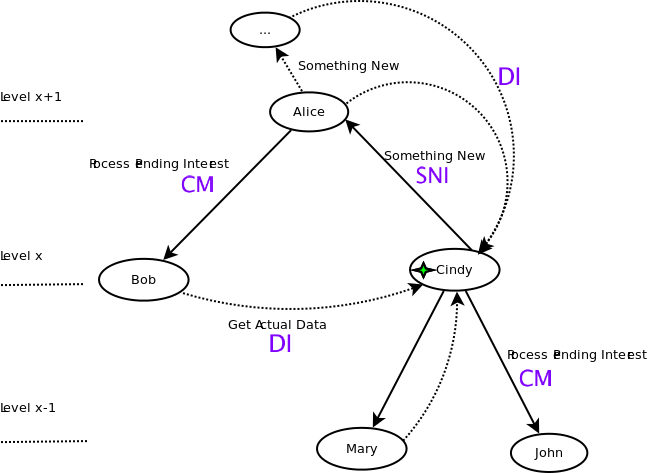
\includegraphics[width=4.5in]{png/tree-synchronization.png}
\caption{Multi-Level Synchronization}
\label{tree_synchronization}
\end{figure}

\section{消息本体获取}

多层控制节点所同步的是控制信息,告诉每一个用户什么时候到什么地方去取数据.

节点得知正确的内容所在的地址(其名称)后,直接向这个地址发interest获取消息本体。这时候使用的是第四种Interest类型:Data Interest.

由于一个节点产生的消息的名字在NDN中是固定不变的,所有人所发送的DI都是相同的.
这样的话,所有其他节点发送的此兴趣包能够充分利用NDN的聚合效果,即NDN会将所有的重复的兴趣包过滤掉,只传输一份到下一跳路由.

同时,当有内容返回时,NDN路由还会缓存这个兴趣包,这样以后的索取此兴趣包的用户就可以在中间路由上得到满足,延迟和链路负载就会大大减少.

\section{鲁棒性和移动性支持}

\begin{figure}
\centering
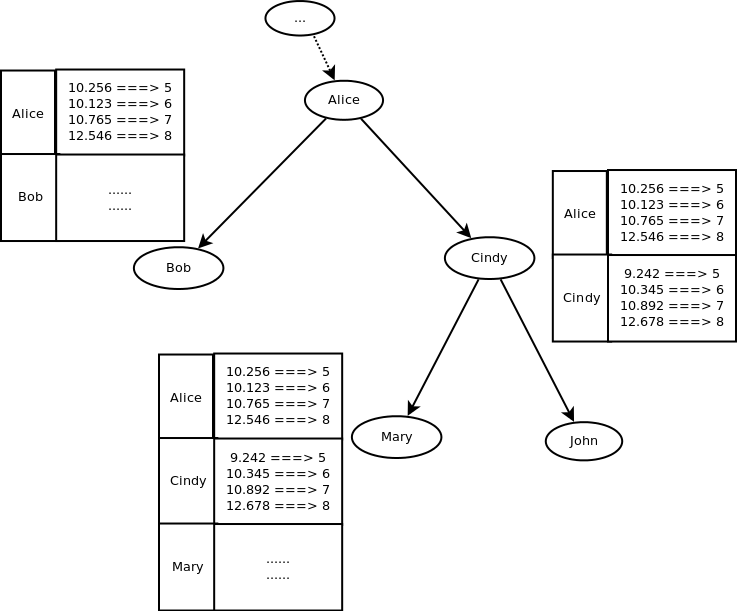
\includegraphics[width=4.5in]{png/mobility.png}
\caption{Robustness and Mobility Support}
\label{mobility_pic}
\end{figure}

\subsection{鲁棒性}
我们的设计是一个分布式的设计,不要求有一个固定的服务器来控制整个系统的同步.
任何一个控制节点出了问题,都可以从其子节点中选出一个来替代它,具有很好的鲁棒性.

在系统稳定时,每个节点都会不停地向其父节点发送心跳包,用以确定父节点的存在性.
如果一个节点因为某种原因下线了,那么其子节点会立刻发现这一点,并且将自己的控制节点清空.
然后,这些子节点会进入控制器产生循环中,向周围广播ANI兴趣包.

按照前述算法,所有的子节点中会产生一个控制器,来代替下线的节点,并继续控制这个组的控制信息的更新与传输.

\subsection{移动性}
当一个节点移动后,其上层节点很有可能共享同一个上层节点。所以还是可以使用其时间标签正常同步。

当节点移动时,有如下三种情况:
\begin{enumerate}
  \item 该节点移动到另一个地方,但是连接到同一个控制节点.
  这种情况下,他仍然会向这个控制节点发送兴趣包以索取控制信息,不受任何影响.
  \item 该节点移动到一个较远的地方,连接到不同的控制节点.
  这个时候,他就不能使用原来的控制节点的标签进行同步了.
  然而,由于多层控制节点是和实际拓扑紧密相关的,很有可能的是,他和新的控制节点共享同一个更上层的控制器.
  这时候,他只需要把自己上层的所有节点的标签发送给新的控制器,就可以保证能继续同步.
  事实上,每个节点最终应该会共享至少顶层控制器.
  \item 该节点移动到一个完全陌生的环境,连顶层节点也不是共享的.
  这可能是由于暂时或永久的隔离引起的.
  考虑这种情况过于极端,因为如果顶层节点不相同,那么实际拓扑也是断的,即没有一条链路是可以让这两个群体相互通讯的.
\end{enumerate}

\section{TreeSync是如何克服ChronoSync的缺点的}

前文介绍了ChronoSync以及其缺点,在本节中,我们将讨论我们的设计是如何克服这些缺点的.

\subsection{并发消息产生}

\begin{figure}
\centering
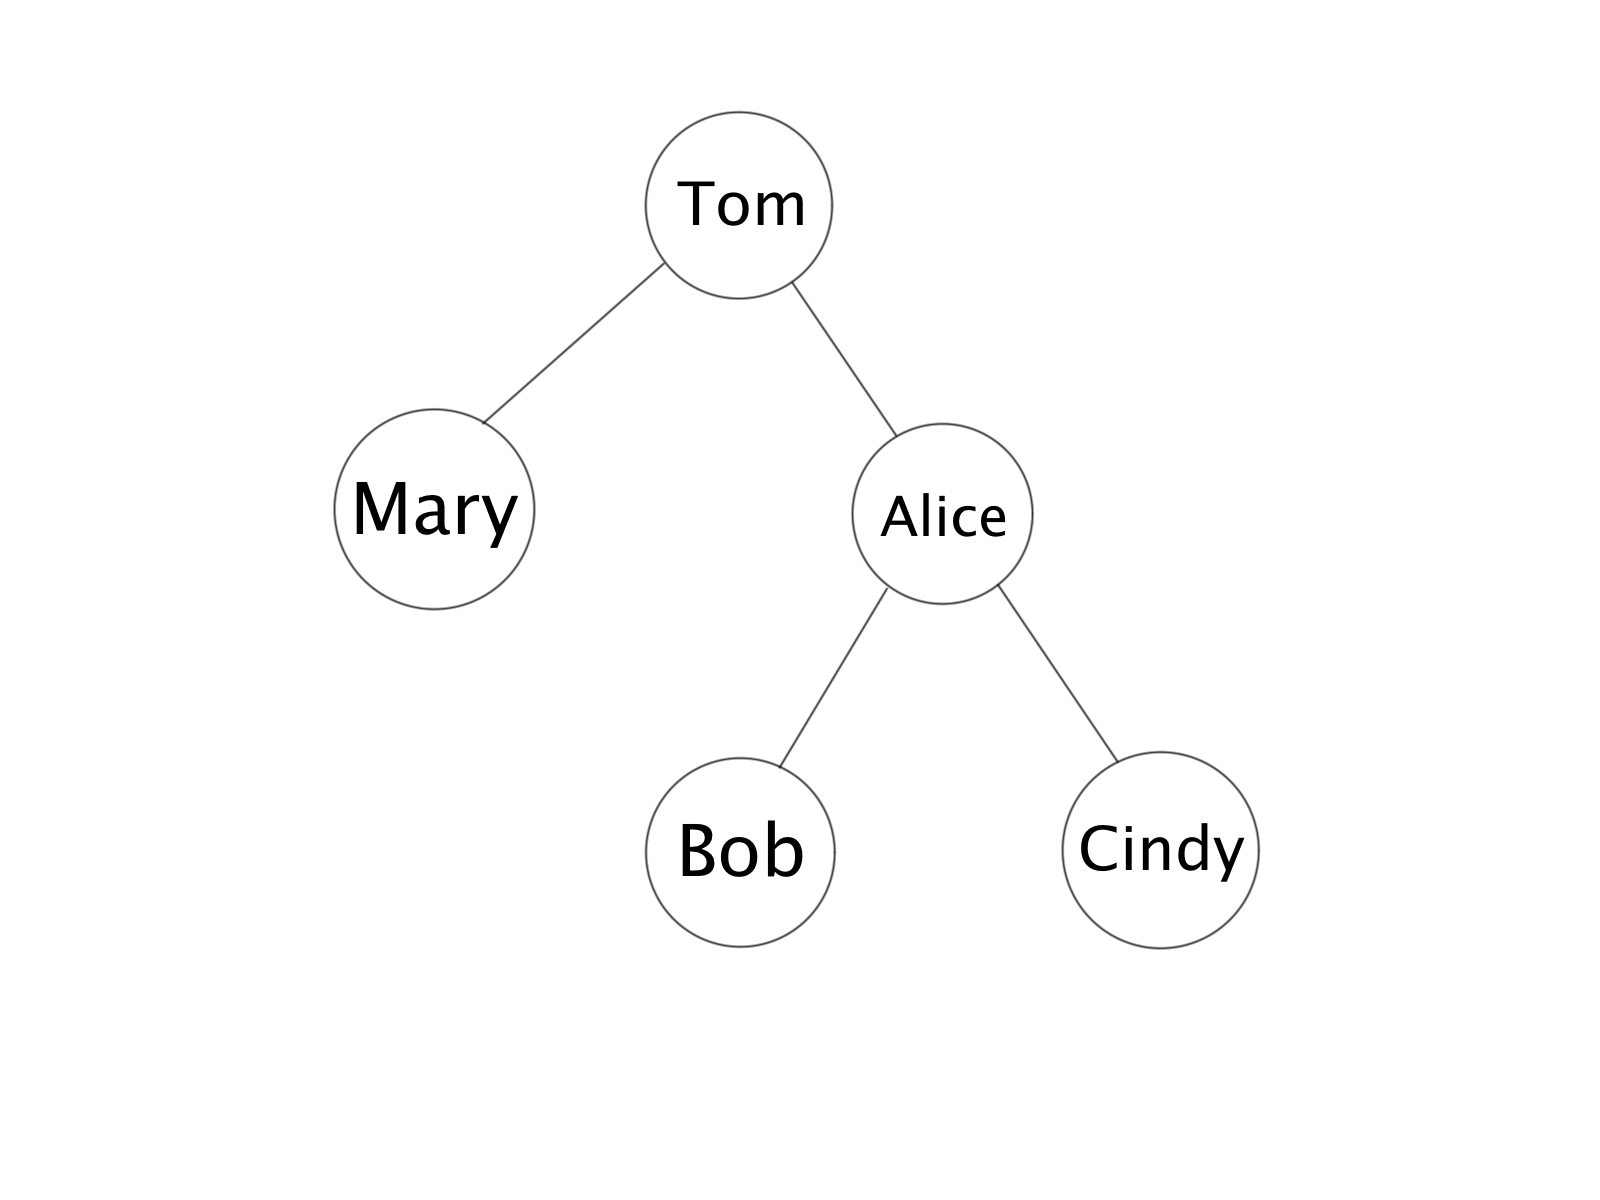
\includegraphics[width=4.5in]{png/merit.png}
\caption{处理并发消息的产生}
\label{merit}
\end{figure}

TreeSync的设计使得他有很强的控制能力.
考虑图\ref{merit},我们考虑如下三种情况:从上层来的两个并发消息;一个上层和一个下层消息;两个从其子节点来的下层消息.

当Tom和Mary同时产生了消息,Tom的消息会直接通过回复Alice的ANI而到达Alice.
当Mary的消息到达Tom,他将会回复Alice的另一个ANI,从而将消息转给Alice.
如果Mary的消息先到达Tom了,Tom还没来的及发送他自己的控制信息,那么他可以将这两个消息打包在一起,同时发送给Alice.

第二种情况中,如果Tom和Bob同时向群中发送消息,无论哪一个先到达Alice,都会由Alice决定消息的顺序,然后将其转发给Cindy.

第三种情况,如果Bob和Cindy同时产生消息,那么它们都会传向Alice.
Alice来对这些消息进行排序,并将控制信息向上和向下传播.

\subsection{扩展性}

ChronoSync没有层级结构,消息是直接广播给群体的,所以没有扩展性,不能用于较大的拓扑.
然而,TreeSync的设计是分层的,每一层都有控制器来掌控所有子节点的控制信息的同步.
因此,消息传递的复杂度相对于群体的人数和拓扑结构是指数下降的.
这保证了TreeSync可以用于更大的拓扑中.
